\chapter{Genetic Algorithm}
A genetic algorithm is a heuristic-based method used for finding optimized solutions for search problems based on natural selection and evolutionary biology.\newline
Here are some genetic algorithm terms that need to be defined in the context of a traveling salesman problem problem:
\begin{itemize}
    \item \textbf{Gene}: a city represented by it's coordinates (x,y)
    \item \textbf{Individual} (also known as “Chromosome”): a route that visits every city only once.
    \item \textbf{Population}: a collection of individuals (a collection of routes)
    \item \textbf{Parents}: two routes that are combined to create a new route
    \item \textbf{Crossover}: a genetic operator used to combine the genetic information of two parents to generate a new offspring
    \item \textbf{Fitness}: a function that is used to evaluate how good each individual is (total distance of a route)
    \item \textbf{Mutation}: a way to introduce variation in our population by randomly altering the genes of an individual
    \item \textbf{Elitism}: a way to carry the best individuals into the next generation
\end{itemize}

\newpage
\section{Advantages and Disadvantages}
\noindent
Advantages of a genetic algorithm compared to conventional methods:
\begin{itemize}
    \item Find a good quality solution in a short amount of time.
    \item A wide range of solutions.
    \item Parallelism, easily adaptable to various problems.
    \item Inherently parallel and easily distributed
\end{itemize}
Disadvantages:
\begin{itemize}
    \item It might not find the most optimal solution to the defined problem in all cases.
    \item It cannot guarantee an optimal solution.
    \item Overfitting (all the individuals have the same genes).
    \item Optimization Time (It usually takes a while to reach the global optimum).
    \item It is hard to choose optimal parameters (generations, population size, mutation chance, etc).
\end{itemize}

\newpage
\section{Architecture}
\begin{figure}[ht]
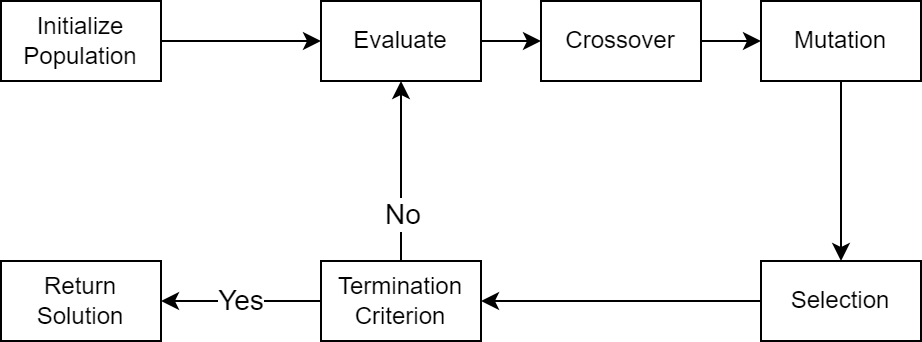
\includegraphics[width=\textwidth]{images/ga_1.png}
\caption{Genetic Algorithm architecture without parallelism}
\end{figure}
In Figure 2.1, we can see the general architecture of the genetic algorithm without parallelism. By doing all of these steps, we simulate natural selection and obtain new individuals each generation. Below, I will explain in detail what every section of the algorithm does.
\subsection{Initialize Population}
Population initialization is the first step in the genetic algorithm process. The initial population is created by generating N number of individuals (N being the size of the population). Each individual is created from a random permutation of genes.
\subsection{Evaluate}
In evaluate we apply the fitness function to the individuals to find out their score. In our case, the fitness calculates the distances between the cities of the individual and returns the sum of the distances.
\subsection{Crossover}
In crossover, we select multiple pairs of individuals with a crossover probability chance. Then we apply an algorithm to combine the genes of both parents to generate a new individual with traits from both parents.
\par
Since we are working with permutations, we can't use the normal two point crossover operator because if we simply switch the genes between two parents, we will have duplicate cities.
\par
We used Partially Mapped Crossover to solve this issue. To build new offspring, we select two random cut points on the parents. Then we take the portion between the cut points and map it onto the other parent, and the rest of the information is exchanged.
\newline
Example:
\newline
$P_{1} = (3\:4\:8\:|\:2\:7\:1\:|\:6\:5)$
\newline
$P_{2} = (4\:2\:5\:|\:1\:6\:8\:|\:3\:7)$
\newline
Firstly, we switch the genes between the crossover points:
\newline
$C_{1} = (X\:X\:X\:|\:1\:6\:8\:|\:X\:X)$
\newline
$C_{2} = (X\:X\:X\:|\:2\:7\:1\:|\:X\:X)$
\newline
Then we can fill the genes for those who have no conflict:
\newline
$C_{1} = (3\:4\:X\:|\:1\:6\:8\:|\:X\:5)$
\newline
$C_{2} = (4\:X\:5\:|\:2\:7\:1\:|\:3\:X)$
\newline
Then, we look for the first X in the first child. In the original parent, it's 8, but 8 is already in this child, so we check the mapping $1 \leftrightarrow 8$ and see again that 1 exists in this child, so we continue checking the next mapping $2\leftrightarrow 1$. 2 isn't anywhere in the first child, so it is valid for the first X. We do the same for the second X. The first option is 6, but 6 already exists, so we check mapping $7 \leftrightarrow 6$, 7 has no conflict, so it occupies the second X. From these results, child 1 is:
\newline
$C_{1} = (3\:4\:2\:|\:1\:6\:8\:|\:7\:5)$
\newline
We repeat the process for child 2 and obtain:
\newline
$C_{2} = (4\:8\:5\:|\:2\:7\:1\:|\:3\:6)$
\newpage
\subsection{Mutation}
In mutation, we select individuals with a mutation probability and perform random gene alterations on them. For the algorithm we used a hybridization of two operators: Partial Shuffle Mutation (PSM) and Reverse Sequence Mutation (RSM)\cite{mutation}.
\newline
\begin{algorithm}
\SetKwInOut{Input}{input}
\SetKwInOut{Output}{output}
\Input{Individual $x=[x_1,x_2,...,x_n]$and $P_m$ is Mutation probability}
\Output{Individual $x=[x_1,x_2,...,x_n]$}
\BlankLine
\emph{Choose two mutation points a and b such that $1 \leq a \leq b \leq n$}\;
\While{$a < b$}{
    \textbf{Permute}($x_a$, $x_b$)\; 
    Choose $p$ a random number between 0 and 1\;
    \If{$p < P_m$}{
        Choose $j$ a random number between 1 and $n$\; 
        \textbf{Permute}($x_a$, $x_j$)\; 
    }
    $a = a + 1$\;  
    $b = b - 1$\;
}
\caption{Hybridizing PSM and RSM Operator (HPRM)\cite{mutation}}\label{algo_disjdecomp}
\end{algorithm}

\subsection{Selection}
The selection stage consists of determining which individuals we keep for the next round of crossover. In our case, we implemented a tournament selection combined with an elitism selection.
\par
In a tournament selection, we select n individuals for the tournament with a selection probability chance. Only the fittest candidate among the selected candidates is chosen and is passed on to the next generation. In this way, many such tournaments take place, and we have our final selection of candidates who move on to the next generation.
\par
The elitism selection consists of selecting some of the best individuals from the previous generation and carrying them over to the next one.
\subsection{Termination Criterion}
The termination condition is usually when a certain number of generations is reached. In our case, because we implemented a parallel genetic algorithm that runs on a network, we keep the clients running until they receive the stop signal from the server or they reach the known optimal solution.
\section{Parameters}
Genetic algorithms include a number of parameters, in our case: population size, mutation probability, crossover probability, elite percentage, selection probability, and migration chance. These parameters usually need to be individually selected for each problem, but I will mention my observations about some of them.
\par
You can choose your population size based on the number of genes in your individual. Usually two times the number of genes is a good start.
\par
A low mutation probability will give better results quickly, but it may lead to premature convergence in a local optimum, while a high probability will lead to a slow convergence speed.
\par
\begin{figure}[H]
\centering
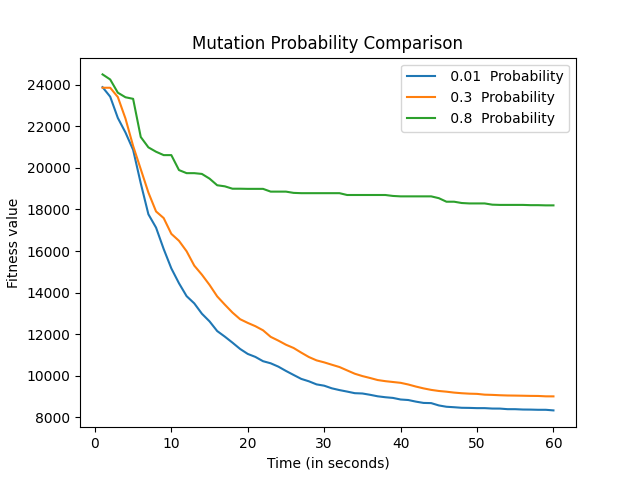
\includegraphics[width=0.9\textwidth]{images/mutation.png}
\caption{Mutation Probability Comparison}
\end{figure}
The crossover probability is pretty similar to the mutation probability. A high probability will lead to slower convergence and values too low will lead to worse results.
\begin{figure}[H]
\centering
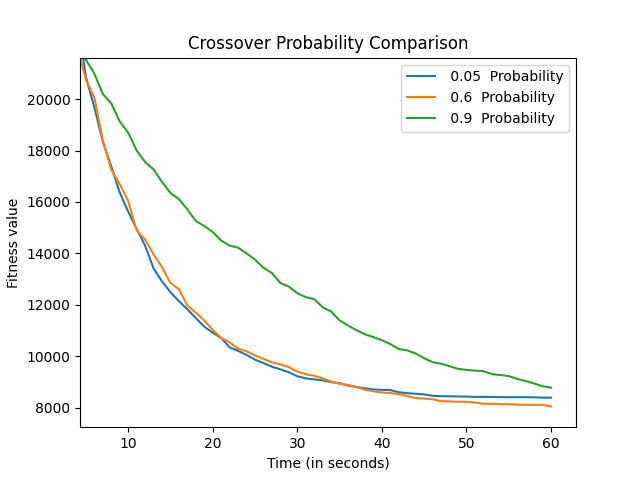
\includegraphics[width=0.9\textwidth]{images/crossover.png}
\caption{Crossover Probability Comparison}
\end{figure}
\par
For the elite percentage, you don't want values too big because in a few generations your entire population will be formed from the same individuals and the same applies to the migration chance. If you use a larger value, the algorithm will converge to a local optimum faster.
\newpage
\section{Parallelism}
It is conceptually pretty straight-forward to adapt a genetic algorithm to a parallel processing one. Each process will operate on an individual subpopulation, performing the stages described above. Periodically, a new stage called migration will run that will share the best individuals with the rest of the processes.
\begin{figure}[ht]
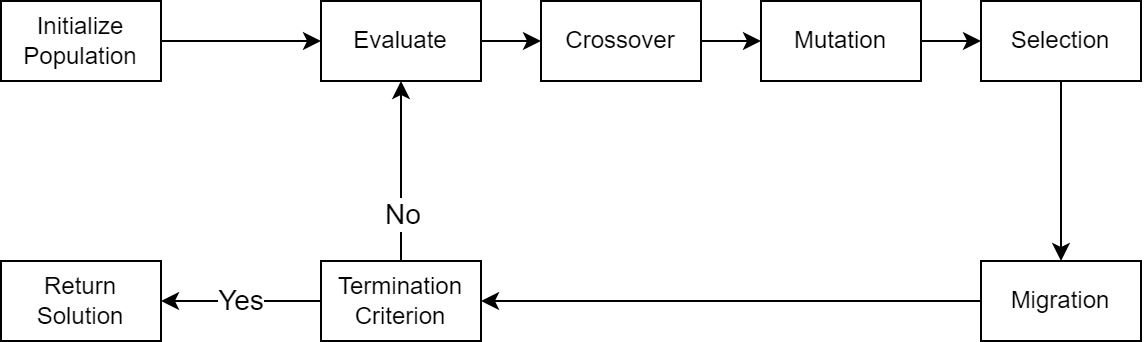
\includegraphics[width=\textwidth]{images/ga_2.png}
\caption{Genetic Algorithm architecture with parallelism}
\end{figure}
\par
Each process generates its own initial population, then each process goes through $N$ generations by performing locally all of the stages described above (Evaluation, Crossover, Mutation, Selection). After these $N$ generations, the processes share their best individuals with the other processes through migration.
\subsection{Migration Operator}
With the implementation of migration, we add another method of affecting the population. The introduction of new individuals will help prevent convergence in a local optimum. During migration, we select some of the best individuals from other processes and replace some of the worst ones from the current process with a migration probability chance. The migration probability chance is critical because it allows us to control the migration's selective pressure. If it is too high, it will lead to faster convergence into a local optimum, and if it is too low, it will lead to fewer individuals migrating and will result in a slower convergence.
\newpage
\subsection{Migration Model}
For our algorithm, we implemented the Island Model. In this model, processes are allowed to share their individuals with any other process, as illustrated in Figure 2.5. There are no restrictions on where an individual may migrate. This model allows more freedom at the cost of more communication overhead and delay.
\begin{figure}[ht]
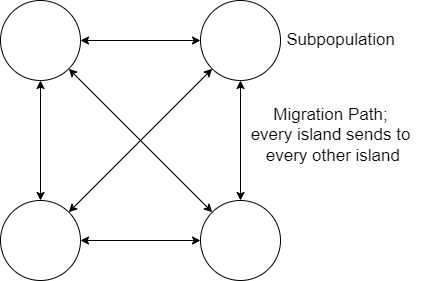
\includegraphics[width=0.6\textwidth]{images/island_model.png}
\caption{Island Model}
\end{figure}